\section{Doo-Sabin} \label{sec:doosabin}

\subsection{Allgemein}

Der Algorithmus Doo-Sabin wurde 1978 von Daniel Doo and Malcolm Sabin entwickelt.
Doo-Sabin ist eine Verallgemeinerung von bi-quadratischen uniformen B-Spline Flächen
und kann auf Netzen mit beliebigen Polygonen arbeiten.
Das verfeinerte Ergebnis nach einem Unterteilungsschritt besteht hauptsächlich
aus Vierecken, an extraordinären Stellen jedoch auch aus beliebigen Polygonen.
Die Kontrollpunkte werden approximiert.
Doo-Sabin erzeugt eine \(C^1\) stetige Fläche.
\cite[S. 79f]{Zorin.subdivcourse}

\subsection{Unterteilungs- und Randregeln}

Ein Unterteilungsschritt lässt sich bei Doo-Sabin in vier Punkte gliedern:
\begin{enumerate}
\item Berechnen der Face Points für jedes Polygon.
\item Berechnen der Edge Points für jede Kante.
\item Berechnen der neuen Vertices (New Points), die das verfeinerte Netz bilden.
\item Erzeugen der neuen Seiten (Vertex Split).
\end{enumerate}

\begin{figure}
\centering
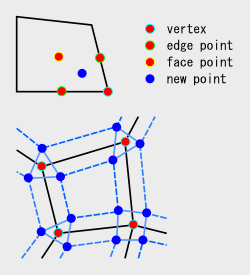
\includegraphics[width=0.4\textwidth]{content/media/sd_doosabin_mask.png}
\caption{Doo-Sabin Maske \cite{Yoshihitoyagi.doosabin}}
\label{fig:sd_doosabin_mask}
\end{figure}
\autoref{fig:sd_doosabin_mask} veranschaulicht den Zusammenhang.

\subsubsection*{Face Point}
Der Face Point wird analog zu Catmull-Clark als Mittelwert der Kontrollpunkte des Polygons
berechnet.

\subsubsection*{Edge Point}
Der Edge Point errechnet sich aus dem Mittelwert der beiden Ecken einer Kante.

\subsubsection*{New Point}
Der New Point ist der Mittelwert aus Face Point, den beiden Edge Points und dem alten Vertex
(siehe \autoref{fig:sd_doosabin_mask}). Das unterteilte Netz besteht nur noch aus diesen New Points.

\subsubsection*{Vertex Split}
Im Gegensatz zu den bisher vorgestellten Algorithmen handelt es sich bei Doo-Sabin nicht um einen
Unterteilungsalgorithmus mit Face Split, sondern mit Vertex Split.
Das bedeutet, dass nicht eine Seite in mehrere Seiten aufgeteilt wird, sondern
jeder Vertex in mehrere Vertices aufgespaltet wird.
Dies ist in \autoref{fig:sd_doosabin_mask} gut erkennbar.
Somit entstehen bei einer Unterteilung mit Doo-Sabin drei unterschiedliche Seitentypen,
die in \autoref{fig:sd_doosabin_faces} markiert sind.
\begin{description}
 \item[Face-Face] Für jede Seite entsteht eine neue Seite.
 Diese erzeugte Seite kann ein beliebiges Vieleck sein.
 \item[Vertex-Face] Für jeden Vertex wird eine neue Seite erstellt.
 Auch diese kann ein beliebiges Vieleck sein.
 \item[Edge-Face] Für jede Kante entsteht immer ein Viereck.
\end{description}
\cite{Yoshihitoyagi.doosabin} \cite{UniCalifornia} \cite{Olsen}

\begin{figure}
\centering
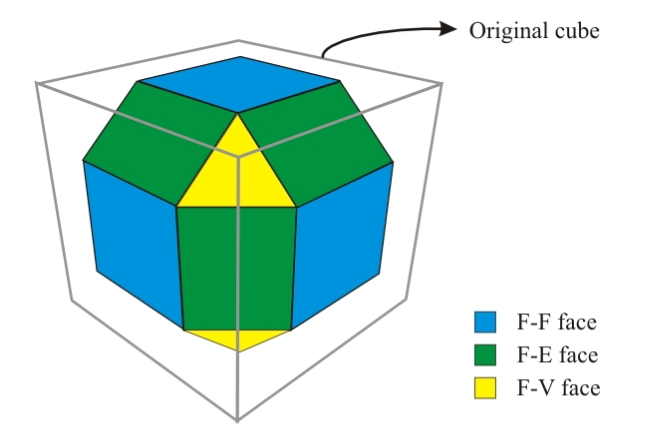
\includegraphics[width=0.6\textwidth]{content/media/sd_doosabin_face_types.jpg}
\caption{Die drei unterschiedlichen Seitentypen, die durch Doo-Sabin erzeugt werden \cite{Olsen}.}
\label{fig:sd_doosabin_faces}
\end{figure}


\subsubsection*{Randregeln}

Die Randregel ist in \autoref{fig:sd_doosabin_boundary} abgebildet.
Es wird jede Randkante durch zwei Vertices ersetzt.
Diese Maske erzeugt am Rand einen quadratischen Spline.
\cite[S. 79f]{Zorin.subdivcourse}

\begin{figure}
\centering
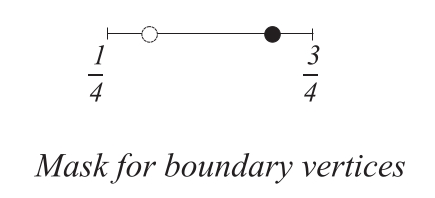
\includegraphics[width=0.4\textwidth]{content/media/sd_doosabin_boundary.jpg}
\caption{Doo-Sabin Randregel \cite[S. 80]{Zorin.subdivcourse}}
\label{fig:sd_doosabin_boundary}
\end{figure}
